% Provenance (never printed): cycle 3 / 6e "La planete Terre" (structure of
% the globe: crust, mantle, core); see sources/book1/PROVENANCE.md. Book 1,
% grade 6, chapter 4.
% Vocabulary guard: "magma" not before g7.2 ("molten rock"); P and S waves,
% Moho, core--mantle boundary and lithosphere belong to Book 2 (g11): the
% waves are told in prose, never defined; "seismometer" is defined in g7.3.
\chapter{L'intérieur de la Terre}\label{ch:g6:inside-the-earth}

Tout au nord-ouest de la Russie, non loin de la frontière avec la Norvège,
un couvercle de métal est soudé sur le sol, au milieu de bâtiments
abandonnés. Dessous, un trou d'environ 23~centimètres de large seulement
descend tout droit sur plus de 12~kilomètres~: c'est le trou le plus
profond jamais creusé. Le forer a pris environ 20~ans. Les foreurs
espéraient aller plus profond encore, mais au fond, la \omterm{def:g3:stones-pebbles-sand:rock}{roche} était à
environ 180~degrés Celsius, presque deux fois plus chaude que prévu~: la
chaleur tordait les trépans et les tubes, et le travail s'est arrêté en
1992. Pourtant, le centre de la Terre est plus de \textbf{500 fois} plus
profond que le fond de ce trou. Comment pouvons-nous savoir ce qu'il y a
là-dessous~?
% ledger: sciam:kola-depth, sciam:kola-180C, earth:Rmean

\begin{omfigure}
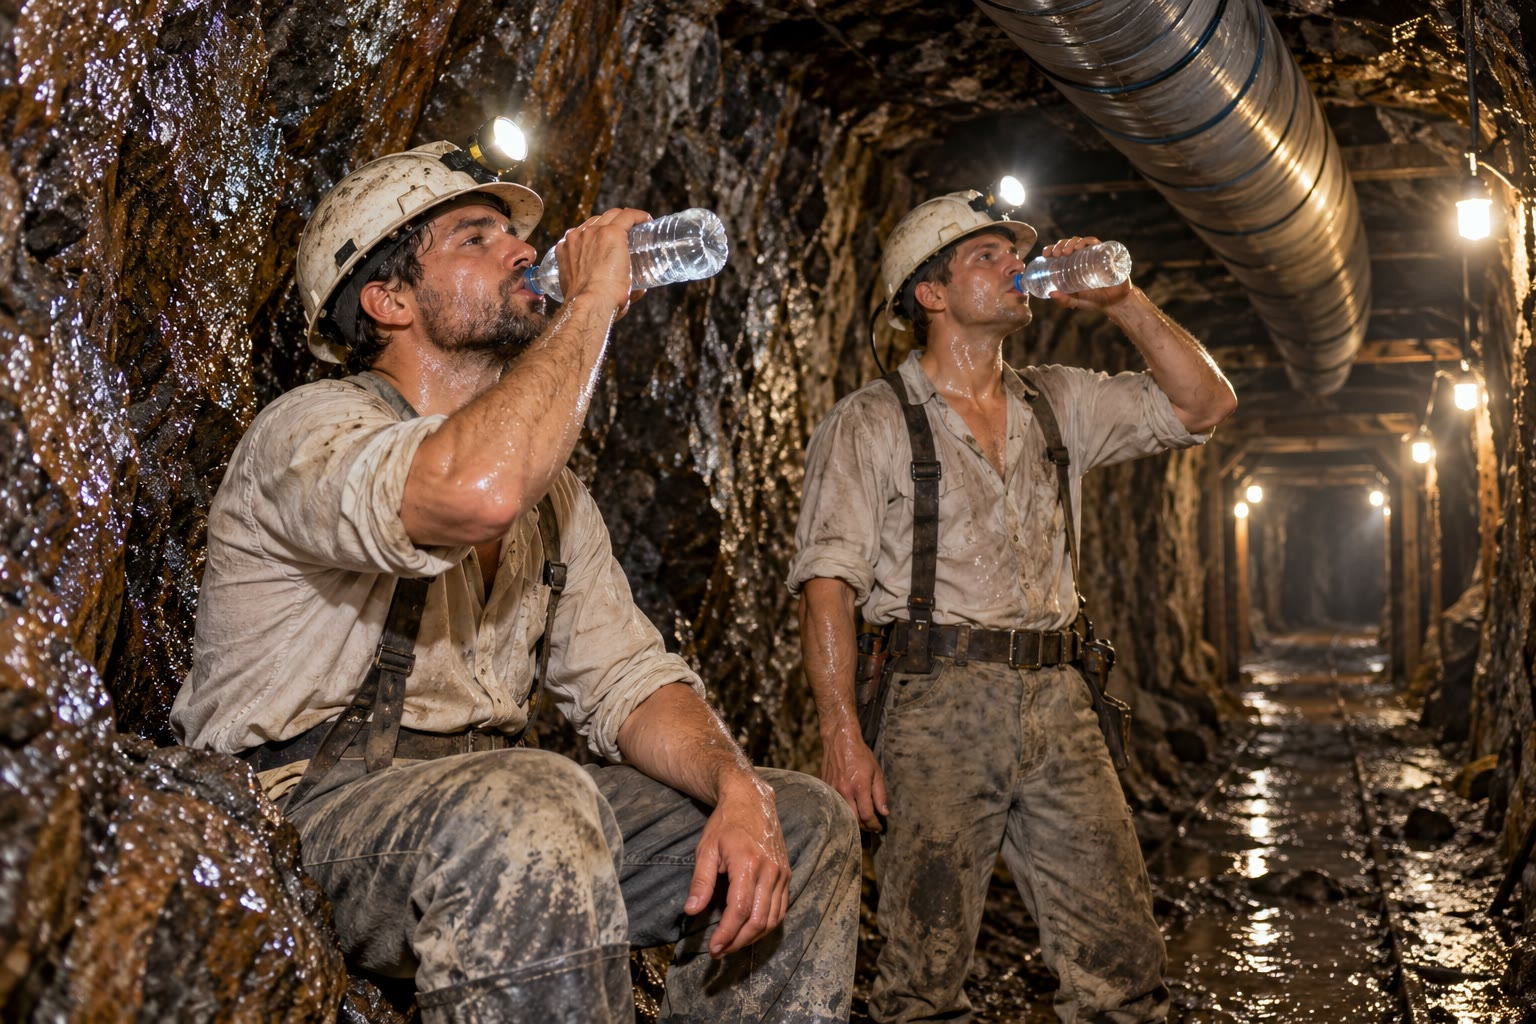
\includegraphics[width=0.62\linewidth]{images/book1/ai/g6-deep-mine.jpg}

{\small Des mineurs boivent dans une galerie chaude, à des kilomètres sous
terre. (Illustration générée par IA.)}
\end{omfigure}

\begin{recall}
La Terre est une \omterm{def:g6:earth-a-planet:planet-types}{planète rocheuse}, une boule d'environ 12\,742~km de
diamètre~: son rayon, de la surface au centre, est d'environ 6371~km
(\cref{ch:g6:earth-a-planet}). Ses \omterm{def:g3:stones-pebbles-sand:rock}{roches} appartiennent à trois familles,
ignées, sédimentaires et métamorphiques (\cref{ch:g6:rocks-and-minerals}).
Sur un \omterm{def:g4:volcanoes-earthquakes-first-look:volcano}{volcan}, la \omterm{def:g3:stones-pebbles-sand:rock}{roche} fondue monte des profondeurs et se répand sous
forme de \omterm{def:g4:volcanoes-earthquakes-first-look:eruption}{lave}~; lors d'un \omterm{def:g4:volcanoes-earthquakes-first-look:earthquake}{séisme}, le sol tremble
(\cref{ch:g4:volcanoes-earthquakes-first-look}).
\end{recall}
% ledger: earth:Rmean

\section{Jusqu'où sommes-nous descendus~?}

Les hommes creusent la Terre depuis longtemps, pour trouver de l'eau, de
la pierre et des métaux. Deux sortes de trous descendent le plus profond.

\textbf{Les mines.} La mine la plus profonde du monde est une mine d'or
près de Johannesburg, en Afrique du Sud. Ses galeries descendent à plus de
4~km sous la surface. Là-dessous, les parois de \omterm{def:g3:stones-pebbles-sand:rock}{roche} atteignent environ
60~degrés Celsius~: on refroidit la mine en y envoyant des milliers de
tonnes de glace mélangée à de l'eau, et grâce à des ventilateurs géants
qui soufflent de l'air dans les galeries.
% ledger: gwr:deepest-mine

\textbf{Les forages.} Un forage est un trou étroit percé depuis la surface
par une machine~; personne n'y descend. Le plus profond est le forage du
récit du début, creusé pour la science dans la péninsule de Kola, au
nord-ouest de la Russie~: 12\,262~mètres, soit environ 12.3~km.
% ledger: sciam:kola-depth

Ces profondeurs paraissent énormes. Comparées à la taille de la Terre,
elles sont minuscules. La figure ci-dessous les montre sur une même bande,
à côté de la plus haute \omterm{def:g1:landscapes-around-us:landform}{montagne}, le mont Everest (8849~m).
% ledger: tht:everest

\begin{omfigure}
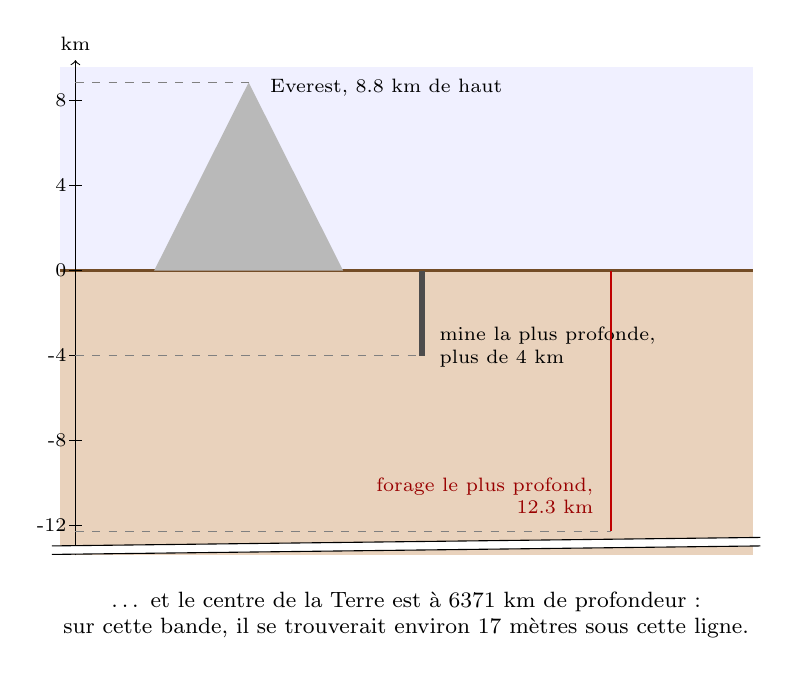
\begin{tikzpicture}[yscale=0.27, xscale=1]
  % sea-level ground and the sky
  \fill[blue!6] (-0.2,0) rectangle (8.6,9.6);
  \fill[brown!35] (-0.2,0) rectangle (8.6,-13.4);
  \draw[thick, brown!60!black] (-0.2,0) -- (8.6,0);
  % depth axis
  \draw[->] (0,-13.4) -- (0,9.9) node[above, font=\scriptsize] {km};
  \foreach \y in {-12,-8,-4,0,4,8} \draw (-0.08,\y) -- (0.08,\y) node[left=2pt, font=\scriptsize] {\y};
  % Everest
  \fill[gray!55] (1.0,0) -- (2.2,8.849) -- (3.4,0) -- cycle;
  \draw[dashed, gray] (0,8.849) -- (2.2,8.849);
  \node[font=\scriptsize, right] at (2.35,8.6) {Everest, 8.8~km de haut};
  % deepest mine
  \draw[line width=2.2pt, black!70] (4.4,0) -- (4.4,-4);
  \draw[dashed, gray] (0,-4) -- (4.4,-4);
  \node[font=\scriptsize, right, align=left] at (4.5,-3.6) {mine la plus profonde,\\ plus de 4~km};
  % Kola borehole
  \draw[line width=0.7pt, red!75!black] (6.8,0) -- (6.8,-12.262);
  \draw[dashed, gray] (0,-12.262) -- (6.8,-12.262);
  \node[font=\scriptsize, left, align=right, red!60!black] at (6.7,-10.6) {forage le plus profond,\\ 12.3~km};
  % break and the centre
  \draw[white, line width=3pt] (-0.3,-13.15) -- (8.7,-12.75);
  \draw (-0.3,-13.35) -- (8.7,-12.95);
  \draw (-0.3,-12.95) -- (8.7,-12.55);
  \node[font=\footnotesize, align=center] at (4.2,-16.2) {\ldots\ et le centre de la Terre est à 6371~km de profondeur~:\\
     sur cette bande, il se trouverait environ 17~mètres sous cette ligne.};
\end{tikzpicture}

{\small Hauteurs et profondeurs dessinées à la même échelle (1~cm pour
3.7~km), à partir du \omterm{def:g4:world-physical-map:altitude}{niveau de la mer}. La coupure de la bande cache presque
tout le chemin jusqu'au centre.}
% ledger: tht:everest, gwr:deepest-mine, sciam:kola-depth, earth:Rmean
\end{omfigure}

\begin{method}[Comparer une profondeur au rayon de la Terre]\label{met:g6:inside-the-earth:percent}
\begin{enumerate}
  \item Écris la profondeur et le rayon dans la même unité (en
        kilomètres).
  \item Divise la profondeur par le rayon, puis multiplie par 100~: tu
        obtiens la profondeur en pourcentage du chemin jusqu'au centre.
  \item Pour dire combien de fois le centre est plus profond, divise le
        rayon par la profondeur.
\end{enumerate}
\end{method}

\begin{example}[Le forage le plus profond]\label{ex:g6:inside-the-earth:kola}
Le forage est profond de 12.3~km et le rayon vaut 6371~km.
$12.3 \div 6371 \approx 0.0019$, et $0.0019 \times 100 = 0.19$~: le forage
a parcouru environ \textbf{0.2~\%} du chemin jusqu'au centre. Dans l'autre
sens, $6371 \div 12.3 \approx 518$~: le centre est plus de 500~fois plus
profond que le fond du trou.

Pour la mine la plus profonde, environ 4~km~: $4 \div 6371 \approx 0.0006$,
soit 0.06~\%~: trois fois moins que le forage.
% ledger: sciam:kola-depth, earth:Rmean, gwr:deepest-mine
\end{example}

Personne n'a donc jamais vu, touché ni prélevé l'intérieur profond de la
Terre. Ce que nous en savons vient d'autres indices, surtout des ondes des
\omterm{def:g4:volcanoes-earthquakes-first-look:earthquake}{séismes} (section~\ref{sec:g6:inside-the-earth:waves}).

\section{Croûte, manteau et noyau}

La Terre est construite en couches, un peu comme un œuf dur~: une fine
coquille fragile, un épais «~blanc~», et un «~jaune~» au milieu.
% ledger: usgs:layers-egg

\begin{omfigure}
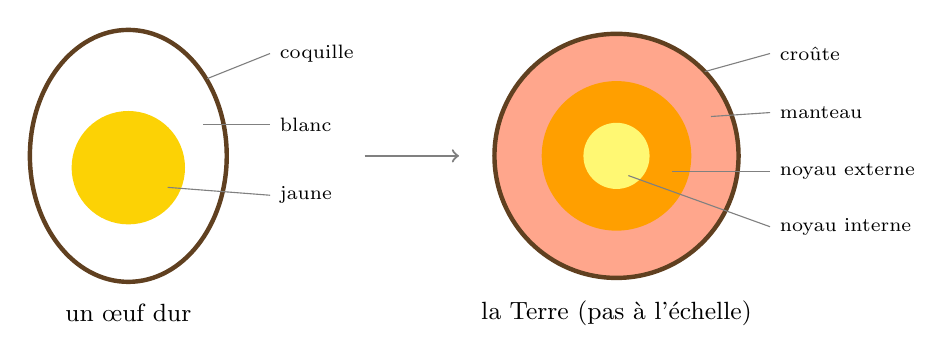
\begin{tikzpicture}
  % a boiled egg cut in half
  \begin{scope}
    \fill[white] (0,0) ellipse (1.25 and 1.6);
    \draw[brown!50!black, line width=1.6pt] (0,0) ellipse (1.25 and 1.6);
    \fill[yellow!70!orange] (0,-0.15) circle (0.72);
    \node[font=\scriptsize, anchor=west] (s) at (1.8,1.3) {coquille};
    \draw[gray] (s.west) -- (1.0,0.98);
    \node[font=\scriptsize, anchor=west] (w) at (1.8,0.4) {blanc};
    \draw[gray] (w.west) -- (0.95,0.4);
    \node[font=\scriptsize, anchor=west] (y) at (1.8,-0.5) {jaune};
    \draw[gray] (y.west) -- (0.5,-0.4);
    \node[font=\small] at (0,-2.0) {un œuf dur};
  \end{scope}
  \draw[->, thick, gray] (3.0,0) -- (4.2,0);
  % the Earth, not to scale
  \begin{scope}[xshift=6.2cm]
    \fill[orange!45!red!45] (0,0) circle (1.55);
    \fill[orange!75!yellow] (0,0) circle (0.95);
    \fill[yellow!55] (0,0) circle (0.42);
    \draw[brown!50!black, line width=1.6pt] (0,0) circle (1.55);
    \node[font=\scriptsize, anchor=west] (c) at (1.95,1.3) {croûte};
    \draw[gray] (c.west) -- (1.12,1.07);
    \node[font=\scriptsize, anchor=west] (m) at (1.95,0.55) {manteau};
    \draw[gray] (m.west) -- (1.2,0.5);
    \node[font=\scriptsize, anchor=west] (o) at (1.95,-0.2) {noyau externe};
    \draw[gray] (o.west) -- (0.7,-0.2);
    \node[font=\scriptsize, anchor=west] (i) at (1.95,-0.9) {noyau interne};
    \draw[gray] (i.west) -- (0.15,-0.25);
    \node[font=\small] at (0,-2.0) {la Terre (pas à l'échelle)};
  \end{scope}
\end{tikzpicture}

{\small La Terre comparée à un œuf dur. Contrairement au jaune, le \omterm{def:g6:inside-the-earth:layers}{noyau} a
deux parties. Sur ce dessin, la \omterm{def:g6:inside-the-earth:layers}{croûte} est beaucoup trop épaisse~; le
dessin à l'échelle vient ensuite.}
% ledger: usgs:layers-egg
\end{omfigure}

\begin{definition}[Les couches de la Terre]\label{def:g6:inside-the-earth:layers}
La Terre est faite de trois couches principales, de la surface au centre~:
\begin{itemize}
  \item la \emph{croûte}\index{croute@croûte}, une fine couche extérieure
        de \omterm{def:g3:stones-pebbles-sand:rock}{roche} solide, épaisse de quelques kilomètres à quelques dizaines
        de kilomètres~;
  \item le \emph{manteau}\index{manteau}, une épaisse couche de \omterm{def:g3:stones-pebbles-sand:rock}{roche}
        solide, chaude et dense, jusqu'à une profondeur d'environ 2900~km~;
  \item le \emph{noyau}\index{noyau}, fait de métal, surtout du fer avec un
        peu de nickel, d'environ 2900~km de profondeur jusqu'au centre. Le
        noyau a deux parties~: le \emph{noyau externe}\index{noyau externe},
        qui est liquide, et le \emph{noyau interne}\index{noyau interne},
        une boule solide au centre, d'environ 1220~km de rayon.
\end{itemize}
% ledger: usgs:layers-egg, usgs:crust-thickness, data:prem, earth:Rmean
\end{definition}

Le dessin ci-dessous montre les couches \emph{à l'échelle}, avec les
limites mesurées grâce aux ondes des \omterm{def:g4:volcanoes-earthquakes-first-look:earthquake}{séismes}.

\begin{omfigure}
\pgfplotstableread{figdata/out/grade-6-earth_layers-disc.dat}\disctab
\pgfplotstablegetelem{0}{r_cm}\of\disctab \let\rE\pgfplotsretval
\pgfplotstablegetelem{1}{r_cm}\of\disctab \let\rOC\pgfplotsretval
\pgfplotstablegetelem{2}{r_cm}\of\disctab \let\rIC\pgfplotsretval
\begin{minipage}[c]{0.43\linewidth}\centering
\begin{tikzpicture}
  \fill[orange!45!red!45] (0,0) circle (\rE cm);
  \fill[orange!75!yellow] (0,0) circle (\rOC cm);
  \fill[yellow!55] (0,0) circle (\rIC cm);
  \draw[brown!50!black, line width=0.45pt] (0,0) circle (\rE cm);
  
  \draw[gray, thin] (-0.25,\rE) rectangle (0.25,\rE-0.12);
  
  \node[font=\scriptsize, align=center, inner sep=0pt] at (0,0) {noyau\\ interne};
  \node[font=\scriptsize, align=center] at (0,1.03) {noyau\\ externe};
  \node[font=\scriptsize] at (0,2.12) {manteau};
  \draw[<-, font=\scriptsize] (1.98,1.98) -- (2.3,2.75) node[above, align=center] {croûte\\ (un trait fin)};
\end{tikzpicture}
\end{minipage}\hfill
\begin{minipage}[c]{0.55\linewidth}\centering
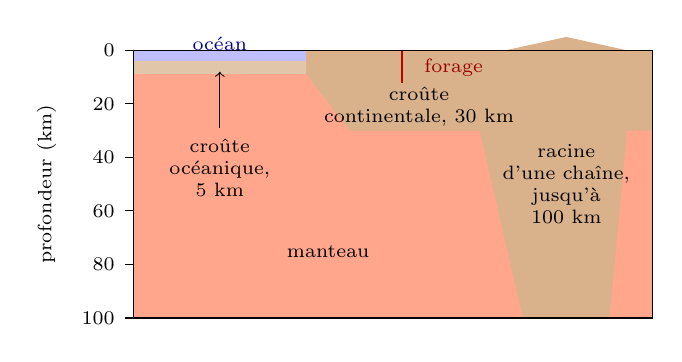
\begin{tikzpicture}[yscale=0.034, xscale=0.55]
  % the top 100 km enlarged: ocean on the left, continent and a range on the right
  \fill[orange!45!red!45] (0,0) rectangle (12,-100);
  \fill[blue!25] (0,0) rectangle (4,-4);
  \fill[brown!45] (0,-4) rectangle (4,-9);                 % oceanic crust 5 km
  \fill[brown!60] (4,0) -- (4,-9) -- (5,-30) -- (8,-30) -- (9,-100) -- (11,-100) -- (11.4,-30) -- (12,-30) -- (12,0) -- cycle;
  \fill[brown!60] (8.6,0) -- (10,5) -- (11.4,0) -- cycle;   % the range (not to scale above ground)
  \draw[red!75!black, line width=0.8pt] (6.2,0) -- (6.2,-12.262);
  \draw[thin] (0,0) rectangle (12,-100);
  \foreach \y in {0,-20,-40,-60,-80,-100} \draw (0,\y) -- (-0.2,\y) node[left, font=\scriptsize] {\pgfmathparse{-\y}\pgfmathprintnumber{\pgfmathresult}};
  \node[font=\scriptsize, rotate=90] at (-2.0,-50) {profondeur (km)};
  \node[font=\scriptsize, align=center] at (2,-44) {croûte\\ océanique,\\ 5~km};
  \draw[->, thin] (2,-29) -- (2,-8);
  \node[font=\scriptsize, align=center] at (6.6,-21) {croûte\\ continentale, 30~km};
  \node[font=\scriptsize, align=center] at (10.0,-50) {racine\\ d'une chaîne,\\ jusqu'à\\ 100~km};
  \node[font=\scriptsize, align=center, red!60!black] at (7.4,-6.5) {forage};
  \node[font=\scriptsize] at (4.5,-75) {manteau};
  \node[font=\scriptsize, blue!60!black] at (2,2.5) {océan};
\end{tikzpicture}
\end{minipage}

\smallskip
{\small À gauche~: la Terre ouverte, à l'échelle~; le petit cadre gris en
haut marque la partie agrandie à droite. À droite~: les 100~premiers km,
agrandis environ 60~fois~: une \omterm{def:g6:inside-the-earth:layers}{croûte} fine sous les \omterm{def:g2:water-on-earth:ocean}{océans}, plus épaisse
sous les \omterm{def:g3:continents-and-oceans:continent}{continents}, encore plus épaisse sous les hautes \omterm{def:g4:world-physical-map:range}{chaînes de
montagnes}~; le forage record en rouge.}
% ledger: data:prem, earth:Rmean, usgs:crust-thickness, sciam:kola-depth (figdata/grade-6/earth_layers.py)
\end{omfigure}

\begin{center}\small
\begin{tabular}{|l|c|c|c|l|}
\hline
\textbf{couche} & \textbf{de (km)} & \textbf{à (km)} & \textbf{épaisseur (km)} & \textbf{faite de} \\
\hline
\omterm{def:g6:inside-the-earth:layers}{croûte} & 0 & 5 à 100 & 5 à 100 & \omterm{def:g3:stones-pebbles-sand:rock}{roche} solide \\
\omterm{def:g6:inside-the-earth:layers}{manteau} & base de la \omterm{def:g6:inside-the-earth:layers}{croûte} & 2891 & environ 2860 & \omterm{def:g3:stones-pebbles-sand:rock}{roche} solide, très chaude \\
\omterm{def:g6:inside-the-earth:layers}{noyau externe} & 2891 & 5150 & environ 2260 & métal liquide \\
\omterm{def:g6:inside-the-earth:layers}{noyau interne} & 5150 & 6371 (centre) & environ 1220 & métal solide \\
\hline
\end{tabular}
\end{center}
% ledger: data:prem, usgs:crust-thickness, usgs:layers-egg, earth:Rmean (figdata/grade-6/earth_layers.py, main table)

\textbf{La \omterm{def:g6:inside-the-earth:layers}{croûte}} est la seule couche sur laquelle nous pouvons marcher et
que nous pouvons creuser. Elle est très fine comparée aux autres~: sous les
\omterm{def:g2:water-on-earth:ocean}{océans}, elle n'a qu'environ 5~km d'épaisseur~; sous les \omterm{def:g3:continents-and-oceans:continent}{continents},
environ 30~km en moyenne~; sous les hautes \omterm{def:g4:world-physical-map:range}{chaînes de montagnes} comme les
Alpes, sa base peut descendre jusqu'à 100~km de profondeur, comme la racine
d'une dent. Même le forage record, profond de 12.3~km, n'a pas traversé la
moitié d'une \omterm{def:g6:inside-the-earth:layers}{croûte} continentale moyenne. Sur le dessin à l'échelle, la
\omterm{def:g6:inside-the-earth:layers}{croûte} est plus fine que le trait qui entoure le disque.
% ledger: usgs:crust-thickness, sciam:kola-depth

\textbf{Le \omterm{def:g6:inside-the-earth:layers}{manteau}} est la couche la plus épaisse~: il va de la base de la
\omterm{def:g6:inside-the-earth:layers}{croûte} jusqu'à 2891~km, environ 45~\% du chemin jusqu'au centre. Sa \omterm{def:g3:stones-pebbles-sand:rock}{roche}
est solide, mais très chaude et plus dense que la \omterm{def:g3:stones-pebbles-sand:rock}{roche} de la \omterm{def:g6:inside-the-earth:layers}{croûte}. Au
fil de millions d'années, la \omterm{def:g3:stones-pebbles-sand:rock}{roche} chaude d'une partie du \omterm{def:g6:inside-the-earth:layers}{manteau} peut se
déformer très lentement, comme une pâte très ferme.
% ledger: data:prem, usgs:layers-egg, usgs:lithosphere-80km

\textbf{Le \omterm{def:g6:inside-the-earth:layers}{noyau}} commence à 2891~km et descend jusqu'au centre. Il n'est
pas fait de \omterm{def:g3:stones-pebbles-sand:rock}{roche}, mais de métal~: un alliage de fer et de nickel, presque
deux fois plus dense que le \omterm{def:g6:inside-the-earth:layers}{manteau}. Sa partie externe est
\emph{liquide}~: un \omterm{def:g2:water-on-earth:ocean}{océan} de métal fondu profond de plus de 2000~km. Sa
partie interne, de 5150~km jusqu'au centre, est une boule \emph{solide} de
métal, d'environ 1220~km de rayon~: environ 70~\% de la largeur de la Lune.
Pendant que la Terre tourne, le métal liquide du \omterm{def:g6:inside-the-earth:layers}{noyau externe} se déplace,
et ce mouvement produit le champ magnétique de la Terre, celui qui fait
tourner l'aiguille d'une boussole.
% ledger: data:prem, usgs:layers-egg, earth:Rmean, planet:Moon.diameter

Plus on descend, plus c'est dense. L'eau a une masse volumique de 1~gramme
par centimètre cube~: la \omterm{def:g3:stones-pebbles-sand:rock}{roche} de la \omterm{def:g6:inside-the-earth:layers}{croûte} est de 2.6 à 2.9 fois plus
dense, la \omterm{def:g3:stones-pebbles-sand:rock}{roche} du bas du \omterm{def:g6:inside-the-earth:layers}{manteau} plus de 5~fois, et le métal du centre
environ 13~fois (voir le graphique ci-dessous). Les matériaux les plus
lourds sont au centre et les plus légers en haut~: la Terre est triée, de
la \omterm{def:g6:inside-the-earth:layers}{croûte} légère au lourd \omterm{def:g6:inside-the-earth:layers}{noyau} de métal.
% ledger: data:prem


\begin{omfigure}
\begin{tikzpicture}
  \begin{axis}[omrecord, width=0.86\linewidth, height=5.4cm,
      xmin=0, xmax=6371, ymin=0, ymax=14,
      xlabel={profondeur sous la surface (km)},
      ylabel={masse volumique (g par cm$^3$)},
      xtick={0,1000,2000,3000,4000,5000,6000},
      scaled x ticks=false, x tick label style={/pgf/number format/1000 sep={}},
      clip=false]
    \fill[orange!45!red!20] (axis cs:24.4,0) rectangle (axis cs:2891,14);
    \fill[orange!75!yellow!35] (axis cs:2891,0) rectangle (axis cs:5149.5,14);
    \fill[yellow!30] (axis cs:5149.5,0) rectangle (axis cs:6371,14);
    \addplot[very thick, black] table[x=depth_km, y=rho] {figdata/out/grade-6-earth_layers-profile.dat};
    \node[font=\scriptsize] at (axis cs:1450,12.5) {manteau};
    \node[font=\scriptsize] at (axis cs:4020,4.5) {noyau externe};
    \node[font=\scriptsize] at (axis cs:5760,4.5) {noyau interne};
    \node[font=\scriptsize, align=left, anchor=west] at (axis cs:80,1.4) {croûte~: 2.6 à 2.9};
  \end{axis}
\end{tikzpicture}

{\small La masse volumique de la Terre à chaque profondeur, d'après un
modèle de référence construit à partir des mesures des \omterm{def:g4:volcanoes-earthquakes-first-look:earthquake}{séismes}. La masse
volumique saute d'environ 5.6 à environ 9.9~g par cm$^3$ là où la \omterm{def:g3:stones-pebbles-sand:rock}{roche}
du \omterm{def:g6:inside-the-earth:layers}{manteau} laisse la place au métal du \omterm{def:g6:inside-the-earth:layers}{noyau}.}
% ledger: data:prem (figdata/grade-6/earth_layers.py, part profile)
\end{omfigure}

\begin{inthelab}[Des couches dans un verre (en classe, avec l'enseignant)]
L'enseignant verse lentement, l'un après l'autre, dans un grand verre~: du
miel, de l'eau colorée avec une goutte d'encre, et de l'huile de cuisine.
Quel que soit l'ordre dans lequel on les verse, au bout d'un moment le miel
se trouve au fond, l'eau au milieu et l'huile en haut~: chaque liquide se
place sous les liquides plus légers et au-dessus des liquides plus denses.
Si on l'agite, le verre devient trouble~; si on le laisse reposer, il se
trie de nouveau. La Terre est disposée en couches de la même façon~: le
matériau le plus dense, le métal du \omterm{def:g6:inside-the-earth:layers}{noyau}, est au centre, et la \omterm{def:g3:stones-pebbles-sand:rock}{roche} la
plus légère est en haut.
\end{inthelab}


\begin{remark}[La croûte est-elle fine~?]\label{rem:g6:inside-the-earth:thin-crust}
Sur un \omterm{def:g3:continents-and-oceans:globe}{globe} d'école de 30~cm de diamètre, la \omterm{def:g6:inside-the-earth:layers}{croûte} continentale (30~km)
aurait environ 0.7~millimètre d'épaisseur, et la \omterm{def:g6:inside-the-earth:layers}{croûte} océanique (5~km)
à peu près l'épaisseur d'une feuille de papier. La \omterm{def:g6:inside-the-earth:layers}{croûte} représente moins
d'un demi pour cent du rayon~: $30 \div 6371 \approx 0.0047$, soit
0.47~\%.
% ledger: usgs:crust-thickness, earth:Rmean
\end{remark}

\section{Comment les ondes des séismes nous apprennent le reste}\label{sec:g6:inside-the-earth:waves}

Si personne n'est descendu à plus de 12~km, comment pouvons-nous dessiner
le \omterm{def:g6:inside-the-earth:layers}{noyau}~? La réponse vient des \omterm{def:g4:volcanoes-earthquakes-first-look:earthquake}{séismes}. Quand un \omterm{def:g4:volcanoes-earthquakes-first-look:earthquake}{séisme} secoue le sol, des
ondes en partent dans toutes les directions et voyagent \emph{à travers}
toute la Terre, comme le bruit d'un coup frappé se propage à travers un
mur. Des instruments, en de nombreux endroits du monde, enregistrent
l'heure d'arrivée de chaque onde (tu les découvriras au
\cref{ch:g7:earthquakes}).
% ledger: data:prem

Les ondes ne voyagent pas à la même vitesse dans tous les matériaux. Quand
elles atteignent la limite entre deux couches, leur vitesse change
brusquement~: certaines ondes rebondissent, d'autres sont déviées en la
traversant, un peu comme la lumière qui entre dans l'eau. En chronométrant
les ondes de nombreux \omterm{def:g4:volcanoes-earthquakes-first-look:earthquake}{séismes}, dans des stations réparties sur tout le
\omterm{def:g3:continents-and-oceans:globe}{globe}, les scientifiques ont trouvé où se trouvent ces limites, et quelles
couches sont solides ou liquides. Les sismologues appellent les deux
principales sortes d'ondes les \emph{ondes P} (les plus rapides, qui
poussent et tirent la \omterm{def:g3:stones-pebbles-sand:rock}{roche}) et les \emph{ondes S} (les plus lentes, qui
la secouent de côté)~; des volumes ultérieurs les étudient de près. Les
ondes S ont une propriété remarquable~: elles ne peuvent pas traverser un
liquide.

\begin{omfigure}
\begin{tikzpicture}
  \begin{axis}[omrecord, width=0.86\linewidth, height=5.4cm,
      xmin=0, xmax=6371, ymin=0, ymax=14.5,
      xlabel={profondeur sous la surface (km)},
      ylabel={vitesse des ondes (km par seconde)},
      xtick={0,1000,2000,3000,4000,5000,6000},
      scaled x ticks=false, x tick label style={/pgf/number format/1000 sep={}},
      clip=false]
    \fill[orange!45!red!20] (axis cs:24.4,0) rectangle (axis cs:2891,14.5);
    \fill[orange!75!yellow!35] (axis cs:2891,0) rectangle (axis cs:5149.5,14.5);
    \fill[yellow!30] (axis cs:5149.5,0) rectangle (axis cs:6371,14.5);
    \addplot[very thick, blue!70!black] table[x=depth_km, y=vp] {figdata/out/grade-6-earth_layers-profile.dat};
    \addplot[very thick, red!75!black] table[x=depth_km, y=vs] {figdata/out/grade-6-earth_layers-profile.dat};
    \node[font=\scriptsize, blue!70!black, anchor=south] at (axis cs:1300,12.9) {ondes P (plus rapides)};
    \node[font=\scriptsize, red!75!black, anchor=north] at (axis cs:1500,6.1) {ondes S (plus lentes)};
    \node[font=\scriptsize, red!75!black, align=center, fill=white, fill opacity=0.8, text opacity=1] at (axis cs:4020,1.9) {ondes S~: 0\\ (liquide)};
    \node[font=\scriptsize] at (axis cs:4020,13.6) {noyau externe};
    \node[font=\scriptsize] at (axis cs:5760,13.6) {noyau interne};
    \node[font=\scriptsize] at (axis cs:1450,1.5) {manteau};
  \end{axis}
\end{tikzpicture}

{\small La vitesse des deux sortes d'ondes sismiques à chaque profondeur,
dans le même modèle de référence. Dans le \omterm{def:g6:inside-the-earth:layers}{noyau externe}, les ondes S
s'arrêtent~: leur vitesse est nulle, parce que le \omterm{def:g6:inside-the-earth:layers}{noyau externe} est
liquide.}
% ledger: data:prem (figdata/grade-6/earth_layers.py, part profile)
\end{omfigure}

Lisons le graphique de gauche à droite~: dans le \omterm{def:g6:inside-the-earth:layers}{manteau}, les deux sortes
d'ondes vont de plus en plus vite avec la profondeur. À 2891~km, les
ondes S disparaissent et les ondes P ralentissent brusquement~: c'est le
haut du \omterm{def:g6:inside-the-earth:layers}{noyau externe} liquide. À 5150~km, les ondes P accélèrent de
nouveau et les ondes S réapparaissent~: c'est le \omterm{def:g6:inside-the-earth:layers}{noyau interne} solide.
% ledger: data:prem

\begin{history}[Inge Lehmann et le noyau interne]
\begin{minipage}[c]{0.72\linewidth}
Au début des années 1930, les sismologues pensaient que la Terre avait deux
couches~: un \omterm{def:g6:inside-the-earth:layers}{manteau} solide autour d'un \omterm{def:g6:inside-the-earth:layers}{noyau} liquide. La sismologue
danoise Inge Lehmann a étudié les ondes d'un fort \omterm{def:g4:volcanoes-earthquakes-first-look:earthquake}{séisme} qui a frappé la
Nouvelle-Zélande en 1929, enregistrées par des stations lointaines.
Certaines ondes arrivaient là où, pour un \omterm{def:g6:inside-the-earth:layers}{noyau} entièrement liquide, elles
n'auraient pas dû arriver du tout. Dans un article de 1936, intitulé
simplement «~P\,$'$~», elle a proposé une explication~: à l'intérieur du
\omterm{def:g6:inside-the-earth:layers}{noyau} liquide se trouve un \emph{\omterm{def:g6:inside-the-earth:layers}{noyau interne} solide}, plus petit, qui
renvoie ces ondes. Elle a écrit modestement que les données étaient
«~tout à fait insuffisantes~» pour en être sûr, mais que l'interprétation
«~semble possible~», et elle a demandé à d'autres chercheurs de la mettre à
l'épreuve. C'est ce qu'ils ont fait, et aujourd'hui le \omterm{def:g6:inside-the-earth:layers}{noyau interne}
solide fait partie de tous les modèles de référence de la Terre, comme
celui qu'utilisent les graphiques de ce chapitre.
% ledger: nbi:lehmann-1936
\end{minipage}\hfill
\begin{minipage}[c]{0.24\linewidth}\centering
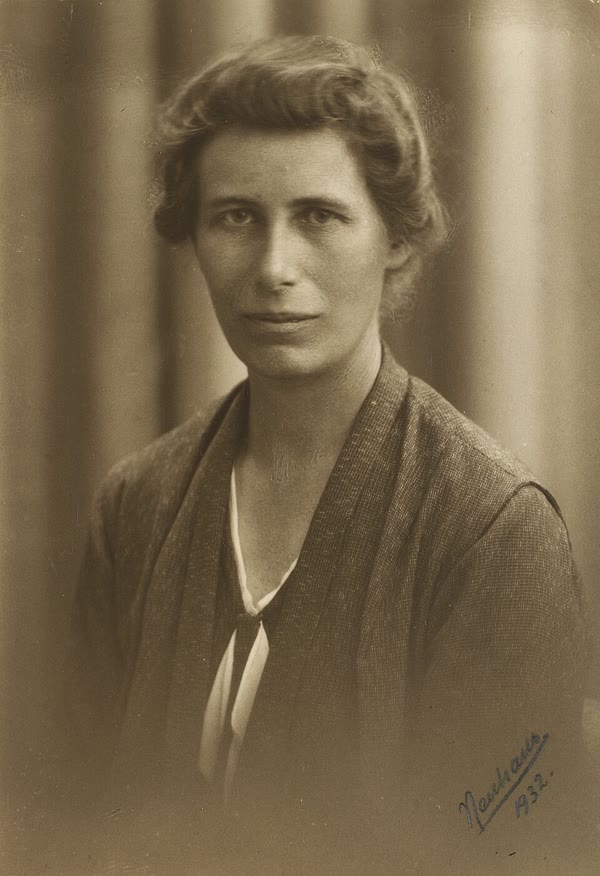
\includegraphics[width=\linewidth]{images/book1/g6-inge-lehmann.jpg}\\[2pt]
{\footnotesize Inge Lehmann en 1932. (Photo~: Even Neuhaus, domaine
public, via Wikimedia Commons.)}
% ledger: commons:inge-lehmann
\end{minipage}
\end{history}

\section{Plus on descend, plus il fait chaud}

Chaque mine profonde et chaque forage profond montrent la même chose~:
plus on descend, plus la \omterm{def:g3:stones-pebbles-sand:rock}{roche} est chaude. Dans la mine la plus profonde,
les parois de \omterm{def:g3:stones-pebbles-sand:rock}{roche} atteignent environ 60~degrés Celsius, à plus de 4~km de
profondeur~; au fond du forage record, à 12.3~km, la \omterm{def:g3:stones-pebbles-sand:rock}{roche} était à environ
180~degrés.
% ledger: gwr:deepest-mine, sciam:kola-180C

Près de la surface, la température monte à un rythme assez régulier. Aux
États-Unis, des scientifiques ont rassemblé les mesures de 284 forages,
pour la plupart plus profonds que 600~m. En moyenne, la température
montait de \textbf{29~degrés par kilomètre} de profondeur~: environ
25~degrés par kilomètre dans l'est du pays et 34 dans l'ouest. Mais ce
rythme varie beaucoup d'un endroit à l'autre~: dans ces forages, il allait
de 6 à 69~degrés par kilomètre.
% ledger: usgs:gradient-29

\begin{omfigure}
\begin{tikzpicture}
  \begin{axis}[omrecord, omdepth, width=0.78\linewidth, height=5.6cm,
      xmin=0, xmax=160, ymin=0, ymax=2,
      xlabel={température de la roche ($^\circ$C)},
      ylabel={profondeur (km)},
      ytick={0,0.5,1,1.5,2},
      yticklabel style={/pgf/number format/fixed},
      legend pos=north east, legend cell align=left,
            legend style={font=\scriptsize},
      clip=false]
    \addplot[forget plot, name path=lo, thin, gray] table[x=t_low, y=depth_km] {figdata/out/grade-6-earth_layers-geotherm.dat};
    \addplot[forget plot, name path=hi, thin, gray] table[x=t_high, y=depth_km] {figdata/out/grade-6-earth_layers-geotherm.dat};
    \addplot[forget plot, gray!20] fill between[of=lo and hi];
    \addplot[forget plot, thick, blue!70!black] table[x=t_east, y=depth_km] {figdata/out/grade-6-earth_layers-geotherm.dat};
    \addplot[forget plot, very thick, black] table[x=t_mean, y=depth_km] {figdata/out/grade-6-earth_layers-geotherm.dat};
    \addplot[forget plot, thick, red!75!black] table[x=t_west, y=depth_km] {figdata/out/grade-6-earth_layers-geotherm.dat};
    \addlegendimage{area legend, fill=gray!20, draw=gray}
    \addlegendentry{6 à 69 $^\circ$C par km~: tous les forages}
    \addlegendimage{thick, blue!70!black}\addlegendentry{25 $^\circ$C par km~: est}
    \addlegendimage{very thick, black}\addlegendentry{29 $^\circ$C par km~: moyenne}
    \addlegendimage{thick, red!75!black}\addlegendentry{34 $^\circ$C par km~: ouest}
  \end{axis}
\end{tikzpicture}

{\small La température en fonction de la profondeur (vers le bas) pour un
sol qui part de 15~$^\circ$C, au rythme moyen (29, en noir), aux moyennes
de l'est et de l'ouest (25 et 34) et sur toute la plage mesurée (6 à 69,
bande grise). Les mesures atteignent environ 2~km.}
% ledger: usgs:gradient-29, planet:Earth.Tmean (figdata/grade-6/earth_layers.py, part geotherm)
\end{omfigure}

\begin{method}[La température à une profondeur donnée]\label{met:g6:inside-the-earth:temperature}
\begin{enumerate}
  \item Prends la température du sol près de la surface.
  \item Multiplie la profondeur, en kilomètres, par le rythme, en degrés
        par kilomètre~: tu obtiens de combien il fait plus chaud.
  \item Additionne les deux. N'utilise ce calcul que sur la plage où le
        rythme a été mesuré~: quelques kilomètres.
\end{enumerate}
\end{method}

\begin{example}[À deux kilomètres de profondeur]\label{ex:g6:inside-the-earth:two-km}
Le sol est à 15~$^\circ$C et le rythme est de 29~degrés par kilomètre.
À 2~km~: $2 \times 29 = 58$ degrés de plus, donc $15 + 58 = 73~^\circ$C~:
plus chaud que le bain le plus chaud, et déjà bien trop chaud pour être
touché.
% ledger: usgs:gradient-29, planet:Earth.Tmean
\end{example}

Peut-on utiliser le même rythme jusqu'au centre~? Non. À 29~degrés par
kilomètre, le centre serait à environ 185\,000~degrés, ce qui est
impossible~: le rythme mesuré dans les premiers kilomètres ne vaut pas en
profondeur, où la hausse doit être beaucoup plus lente. Les scientifiques
estiment la température du \omterm{def:g6:inside-the-earth:layers}{noyau} d'une autre façon~: au laboratoire, ils
écrasent de minuscules grains de fer entre deux diamants, jusqu'à des
millions de fois la pression de l'air, et ils les chauffent avec des lasers
jusqu'à ce qu'ils fondent. Ils ont ainsi trouvé qu'à la limite du \omterm{def:g6:inside-the-earth:layers}{noyau
interne} solide, la température est d'environ
\textbf{6000~degrés Celsius}, et pourtant le fer du \omterm{def:g6:inside-the-earth:layers}{noyau interne} reste
solide, parce que la pression qui y règne, environ 3.3~millions de fois la
pression de l'air, l'empêche de fondre.
% ledger: esrf:core-6000C, usgs:gradient-29

\begin{remark}[Chaud, et pourtant solide]\label{rem:g6:inside-the-earth:pressure}
Quand on comprime fortement une substance, elle ne fond qu'à une
température plus élevée. Le \omterm{def:g6:inside-the-earth:layers}{manteau} est très chaud, et pourtant il reste
solide~; le \omterm{def:g6:inside-the-earth:layers}{noyau externe} est liquide~; le \omterm{def:g6:inside-the-earth:layers}{noyau interne}, encore plus
chaud, est de nouveau solide, parce que c'est lui qui est le plus
comprimé. Ce qui fond ou non dépend de la température \emph{et} de la
pression.
% ledger: esrf:core-6000C, data:prem
\end{remark}

\section{Exercices}

\begin{exercise}[$\star$]\label{exo:g6:inside-the-earth:1}
Nomme les quatre couches de la Terre dans l'ordre, de la surface au
centre. Laquelle est liquide~? Lesquelles sont faites de métal~?
\end{exercise}

\begin{exercise}[$\star$]\label{exo:g6:inside-the-earth:2}
Vrai ou faux~? Corrige les phrases fausses.
(a) La \omterm{def:g6:inside-the-earth:layers}{croûte} est plus épaisse sous les \omterm{def:g2:water-on-earth:ocean}{océans} que sous les \omterm{def:g3:continents-and-oceans:continent}{continents}.
(b) Le \omterm{def:g6:inside-the-earth:layers}{noyau} est fait de \omterm{def:g3:stones-pebbles-sand:rock}{roche}.
(c) Le \omterm{def:g6:inside-the-earth:layers}{noyau interne} est solide.
(d) Le forage le plus profond jamais creusé mesure environ 12~km.
\end{exercise}

\begin{exercise}[$\star$]\label{exo:g6:inside-the-earth:3}
Utilise le tableau des couches. (a) À quelle profondeur commence le
\omterm{def:g6:inside-the-earth:layers}{noyau}~? (b) À quelle profondeur commence le \omterm{def:g6:inside-the-earth:layers}{noyau interne}~? (c) Quelle est
l'épaisseur du \omterm{def:g6:inside-the-earth:layers}{noyau externe}~?
\end{exercise}

\begin{exercise}[$\star$]\label{exo:g6:inside-the-earth:4}
On compare souvent la Terre à un œuf dur. Recopie et complète~: «~La
coquille est comme la \ldots, le blanc est comme le \ldots{} et le jaune
est comme le \ldots{}. Mais contrairement au jaune, le \ldots{} a deux
parties~: un \ldots{} liquide et un \ldots{} solide.~»
\end{exercise}

\begin{exercise}[$\star\star$]\label{exo:g6:inside-the-earth:5}
Le mont Everest culmine à 8.849~km et le rayon de la Terre est de
6371~km. En pourcentage du rayon, quelle est la hauteur de l'Everest~?
Arrondis à deux décimales. Vue de loin, la surface de la Terre est-elle
très bosselée~?
\end{exercise}

\begin{exercise}[$\star\star$]\label{exo:g6:inside-the-earth:6}
La \omterm{def:g6:inside-the-earth:layers}{croûte} continentale a 30~km d'épaisseur en moyenne et la \omterm{def:g6:inside-the-earth:layers}{croûte}
océanique 5~km. (a) Combien de fois la \omterm{def:g6:inside-the-earth:layers}{croûte} continentale est-elle plus
épaisse~? (b) Sous une haute \omterm{def:g4:world-physical-map:range}{chaîne de montagnes}, la \omterm{def:g6:inside-the-earth:layers}{croûte} peut atteindre
100~km. Combien de fois plus épaisse que la \omterm{def:g6:inside-the-earth:layers}{croûte} océanique est-elle
alors~?
\end{exercise}

\begin{exercise}[$\star\star$]\label{exo:g6:inside-the-earth:7}
Dans une région, le sol est à 12~$^\circ$C et la température monte de
25~degrés par kilomètre. Quelle est la température (a) à 1~km, (b) à
1.5~km, (c) à 2~km~?
\end{exercise}

\begin{exercise}[$\star\star$]\label{exo:g6:inside-the-earth:8}
Dans un forage, la \omterm{def:g3:stones-pebbles-sand:rock}{roche} est à 14~$^\circ$C près de la surface et à
74~$^\circ$C à 2~km de profondeur. De combien de degrés la température
monte-t-elle par kilomètre~? Ce rythme est-il compris entre les moyennes
de l'est et de l'ouest des mesures du chapitre~?
\end{exercise}

\begin{exercise}[$\star\star$]\label{exo:g6:inside-the-earth:9}
Utilise le graphique des vitesses des ondes. (a) Quelle est la vitesse des
ondes P juste au-dessus du \omterm{def:g6:inside-the-earth:layers}{noyau}, vers 2890~km, et juste sous le haut du
\omterm{def:g6:inside-the-earth:layers}{noyau}~? (b) Entre quelles profondeurs la vitesse des ondes S est-elle
nulle~? (c) Qu'est-ce que cela nous apprend sur cette couche~?
\end{exercise}

\begin{exercise}[$\star\star$]\label{exo:g6:inside-the-earth:10}
Le forage record est profond de 12.3~km. (a) Quel pourcentage d'une \omterm{def:g6:inside-the-earth:layers}{croûte}
continentale moyenne (30~km) a-t-il traversé~? (b) A-t-il atteint le
\omterm{def:g6:inside-the-earth:layers}{manteau}~?
\end{exercise}

\begin{exercise}[$\star\star\star$]\label{exo:g6:inside-the-earth:11}
Léo dit~: «~Près de la surface, la température monte de 29~degrés par
kilomètre~; donc au centre, à 6371~km de profondeur, elle doit être de
$15 + 29 \times 6371$ degrés.~» (a) Calcule le nombre de Léo. (b) Compare-le
avec la température trouvée au laboratoire pour la limite du \omterm{def:g6:inside-the-earth:layers}{noyau
interne}. (c) Qu'est-ce qui ne va pas dans le raisonnement de Léo~?
\end{exercise}

\begin{exercise}[$\star\star\star$]\label{exo:g6:inside-the-earth:12}
La Terre entière a une masse volumique moyenne d'environ 5.5~grammes par
centimètre cube (\cref{ch:g6:earth-a-planet}), mais les \omterm{def:g3:stones-pebbles-sand:rock}{roches} de la
\omterm{def:g6:inside-the-earth:layers}{croûte} n'ont qu'une masse volumique de 2.6 à 2.9. (a) Qu'est-ce que cela
nous apprend sur les matériaux plus profonds~? (b) Utilise le graphique des
masses volumiques~: dans quelles couches la masse volumique est-elle
partout supérieure à 5.5~? (c) Pourquoi est-il logique que le métal lourd
se trouve au centre et non à la surface~?
\end{exercise}

\section{Problème~: Un voyage au centre, à l'échelle}

\begin{problem}[{Problème du week-end --- une Terre en maquette de 2~mètres de diamètre~: les
couches, les trous les plus profonds et l'intérieur chaud, à l'échelle}]
\label{pb:g6:inside-the-earth:1}
% ledger: earth:Rmean, data:prem, usgs:crust-thickness, sciam:kola-depth, tht:everest, usgs:gradient-29, gwr:deepest-mine, esrf:core-6000C
Pour la fête de l'école, une classe construit une maquette de la Terre
coupée en deux, aussi grande que possible~: la face plane de la
demi-boule est un disque de 2~mètres de diamètre, peint avec les couches.
Tout doit être à l'échelle. Utilise~: rayon de la Terre 6371~km~; haut du
\omterm{def:g6:inside-the-earth:layers}{noyau externe} 2891~km~; haut du \omterm{def:g6:inside-the-earth:layers}{noyau interne} 5150~km~; \omterm{def:g6:inside-the-earth:layers}{croûte}
continentale 30~km~; \omterm{def:g6:inside-the-earth:layers}{croûte} océanique 5~km~; Everest 8.849~km~; forage
record 12.3~km.

\medskip
\noindent\textbf{Partie I --- La maquette.}
\begin{enumerate}
  \item Quel est le diamètre de la Terre, en kilomètres~? Écris le diamètre
        de la maquette en millimètres.
  \item Combien de kilomètres de la vraie Terre représente 1~millimètre de
        la maquette~? (Divise le diamètre réel par le diamètre de la
        maquette.)
  \item Sur la maquette, quelle est la hauteur de l'Everest, en
        millimètres~? Arrondis à une décimale.
  \item Quelle est la profondeur du forage record sur la maquette~?
        Compare-la avec la distance de la surface au centre de la maquette.
\end{enumerate}

\medskip
\noindent\textbf{Partie II --- Les couches.}
\begin{enumerate}[resume]
  \item À quelle distance sous la surface de la maquette les élèves
        doivent-ils peindre le haut du \omterm{def:g6:inside-the-earth:layers}{noyau externe}~? Arrondis au
        millimètre.
  \item Même question pour le haut du \omterm{def:g6:inside-the-earth:layers}{noyau interne}. Quel est le rayon du
        \omterm{def:g6:inside-the-earth:layers}{noyau interne} sur la maquette~?
  \item Quelle couche occupe le plus de place le long d'un rayon de la
        maquette~: le \omterm{def:g6:inside-the-earth:layers}{manteau}, le \omterm{def:g6:inside-the-earth:layers}{noyau externe} ou le \omterm{def:g6:inside-the-earth:layers}{noyau interne}~? Donne
        son épaisseur sur la maquette.
  \item Quelle épaisseur faut-il peindre pour la \omterm{def:g6:inside-the-earth:layers}{croûte} continentale~?
        Arrondis à une décimale. Est-ce facile avec un pinceau~?
\end{enumerate}

\medskip
\noindent\textbf{Partie III --- L'intérieur chaud.}
\begin{enumerate}[resume]
  \item Les élèves écrivent la température à 2~km, avec un sol à
        15~$^\circ$C et 29~degrés par kilomètre. Qu'écrivent-ils~? À quelle
        distance sous la surface de la maquette se trouvent 2~km~?
  \item La mine la plus profonde descend à plus de 4~km. Sur la maquette,
        la mine est-elle plus ou moins profonde que le forage record~? De
        combien de millimètres environ~?
  \item Près de la limite du \omterm{def:g6:inside-the-earth:layers}{noyau interne}, l'étiquette indique «~environ
        6000~$^\circ$C, solide~». Un visiteur est surpris~: pourquoi le
        \omterm{def:g6:inside-the-earth:layers}{noyau externe} est-il liquide, alors que le \omterm{def:g6:inside-the-earth:layers}{noyau interne}, encore
        plus chaud, est solide~?
  \item La \omterm{def:g6:inside-the-earth:layers}{croûte} océanique est la couche la plus fine. Quelle épaisseur
        doit-elle avoir sur la maquette, en millimètres~? Arrondis à deux
        décimales, et compare-la avec l'épaisseur d'une feuille de papier
        (environ 0.1~mm).
\end{enumerate}
\end{problem}
